\documentclass[11pt]{article}
\usepackage{amsfonts}
\usepackage{amssymb,amsmath}
\usepackage{fullpage}
\usepackage{graphicx}
\usepackage[usenames]{color}
\setlength{\oddsidemargin}{0pt}
\setlength{\evensidemargin}{0pt}
\setlength{\textwidth}{6.0in}
\setlength{\topmargin}{0in}
\setlength{\textheight}{8.5in}

\newtheorem{Thm}{Theorem}
\newtheorem{Lem}[Thm]{Lemma}
\newtheorem{Cor}[Thm]{Corollary}
\newtheorem{Prop}[Thm]{Proposition}
\newtheorem{Claim}[Thm]{Claim}
\newtheorem{lemma}{Lemma}
\newtheorem{Observation}{Observation}
\newtheorem{theorem}{Theorem}
\newenvironment{proof}{\noindent {\sc Proof:}}{$\Box$ \medskip}

\title{Boosting and Switching experts for object tracking}

\begin{document}

\maketitle

\newcommand{\bx}{{\bf x}}
\newcommand{\by}{{\bf y}}

\section{Introduction}
There has been significant success with using boosting, specifically
``online boosting'' for object tracking in video~\cite{}. While there
has been significant success, no theoretical guarantees have been
associated with this mkethod. It is therefor difficult to understand
why the method fails when it does and how to improve it to reduce
failures.

In this paper we construct an alternative algorithm to that
of~\cite{}, and give theoretical guarantees to it's performance.

Tracking algorithms are composed of two main parts: an appearance
model and a dynamics model. In this paper we concentrate on the
appearance model.

The appearance model is a {\em score function} that is used to
identify the location of the tracked object. The score distribution we
would like to have is a sharp peak surrounded by much lower
scores. In order to have confidence in the location of the peak we
want the difference between the max value and the values far from the
max to be {\em statistically significant}. Note that statistical
significance is used here as a stand in for ``ground truth'' which is
not usually available.

We propose two complementary methods for combining score functions:
\begin{itemize}
\item {\bf Boosting:} We use boosting to combine so-called {\em weak
  score functions} into a single {\em strong score function}
\item{\bf Sleeping experts:} We use an online algorithm for {\em
  switching among a small set of experts} to allow different scoring
  functions to be used at differen times, and to combine different
  trackers that are centered at different locations and/or use
  multiple resolutions. Note that the experts in this part are
  equivalent to the {\em strong} score functions of the boosting method.
\end{itemize}

The rest of the paper is organized as follows. We start by describing
the method for boosting score functions. We then give the details of
the boosting process and it's justification. We then describe details
that are specific to the tracking process. Finally we describe how
sleeping experts are used to combine different strong score functions.

\section{Boosting significance}

\newcommand{\vx}{\vec{x}}
\newcommand{\vxmax}{\vec{x}_{\mbox{max}}}
\newcommand{\wmax}{w_{\mbox{max}}}
\newcommand{\smax}{s_{\mbox{max}}}
\newcommand{\sdecoy}{s_{\mbox{decoy}}}

A score function $F$ is mapping of a region of an image which we call the
{\em appearance window} to a real number. Let $w(\vx)$ denote the
appearance window (for example, a $20 \times 20$ grey-level matrix)
centered at the location defined by the vector $\vx$. The score that
the score function $F$ associates with the location $\vx$ is denoted
by $F(w(\vx))$.

Given an image window, we quantify the performance of the score
function as follows:
\begin{enumerate}
\item Find the location where the score is maximized, denote the
  location by $\vxmax$ and the window at that location by
  $\wmax=w(\vxmax)$. The maximal score is therefor
  $\smax \doteq F(\wmax)$.\footnote{It might be better to use the maximum of an
    {\em average} over a small neigborhood of scores such as a $2
    \times 2$ or a $3 \times 3$ square.}
\item compute the score for all locations $\vx$ in the image window
  which are sufficiently far from $\vxmax$. We call the window that
  achieves the highest score in this set the {\em decoy} window
  because this window is the most likely one to distract the tracker
\[
\sdecoy = \max \left\{ F(w(\vx)) \left\| d(\vx,\vxmax)>r \right. \right\}
\]

The performance of the scoring function is measured by $\smax -
\sdecoy$. In order to see if this difference is significant we need to
compare it to a ``Null'' distribution. We construct this null
distribution as follows:
\begin{itemize}
\item We estimate the standard-deviation of the score function $F$
  using the empirical variance of the score function $F$ in the image
  window.
\item We make the assumption that the scores $F(w)$ are drawn IID from
  a normal distribution with some mean $\mu$ and the estimated
  standard deviation.
\item Suppose the total number of locations for which the score is
  calculated is $N$. The null distribution over the score difference
  $\smax - \sdecoy$ is the distribution resulting from taking $N$ IID
  samples from the normal distribution and then considering the
  difference between the largest and the second largest values. We
  need to find out what is the form of this distribution.
\end{itemize}
\end{enumerate}


\section{Definition of the visual regions}

\begin{figure*}[t]
\centering
  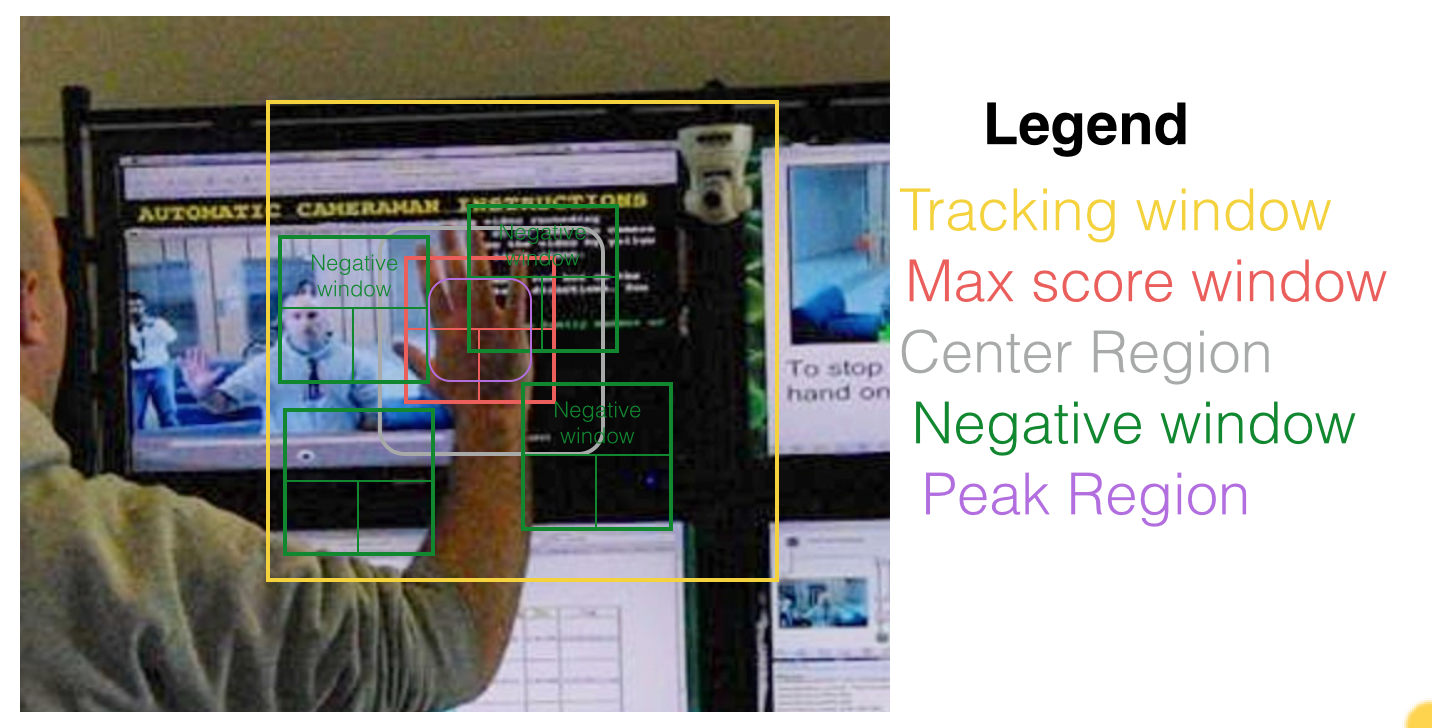
\includegraphics[width=0.9\textwidth] {Figures/TrackingRegions.png}
\label{fig:TrackingRegions}
\caption{The windows involved in training the tracker}
\end{figure*}

We now define the goal of the apearance model training
algorithm.

We denote $w(\vx)$ the appearance window centered at the location
$\vx=(x,y)$. The point $\vx$ is constrained to a region of the image
that we call the {\bf tracking window}. See
Figure~\ref{fig:TrackingRegions} for a depiction of the tracking
region and the other regions defined below.

We score all windows whose center is inside the tracking region and
define the window with the maximal score as the {\bf max window} and
denote it by $\wmax$. We then define a region around the center of the
max window which we call the {\bf center region}. The center region
corresponds, intuitively, to the desired shape of the peak. More on
that below.

The training examples are defined as pairs of windows. The first
window in each pair is the max window $\wmax$. The second is a window
$w(\vx)$ such that $\vx$ is not in the center region. The score of a pair


\subsection{The effect of the size of the center region}
Choosing the size of the center region is a tradeoff between accuracy
and robustness. Setting it to be small will generate a tracker which
can localize more accurately, possibly at the cost of failing to track
more easily. On the other hand, setting the center window to be large,
will generate a tracker that is less likely to loose tracking, but the
location of the tracking point might slide from place to place on the
target. A combination of sizes and resolution is probably the best way
to create a tracker that is both robust and accurate.




We now come to the first novelty in our approach. In the standard
framework for boosting the training set contains the {\em ground
  truth} label for each instance. However, in the tracking problem no
such ground truth is available. Instead, we propose an approach which
measures the quality of a base function using the {\em statistical
  significance} of the outputs of the function.

To define statistical significance we need to first define a {\em null
  hypothesis}. Our null hypothesis is that the values of $F(w)$ are
independently drawn from a normal distribution with unknown, but
fixed, mean and variance. We will be looking for a function $F$ which
defines a sinstatistically significant 

 whose
value are statistically significant and which is {\em coherent} with
the current scoring function.

We denote by $w(x,y)$ the window around the center point $(x,y)$.
We use the euclidean distance: 
\[
d((x_1,y_1),(x_2,y_2)) = \sqrt{(x_1-x_2)^2+(y_1-y_2)^2}
\]
\newcommand{\dmin}{d_{\mbox{min}}}
\newcommand{\xin}{x_{\mbox{in}}}
\newcommand{\xout}{x_{\mbox{out}}}
\newcommand{\yin}{y_{\mbox{in}}}
\newcommand{\yout}{y_{\mbox{out}}}

We define a ``minimum distance'' parameter $\dmin$ which will be
around the size of the window $w$. Setting $\dmin$ smaller will make
for a more accurate and less robust scoring function.

\section{Boosting and Sanov}
Let the input space be $X=\{-1,+1\}^d$, where $d$ corresponds to the
number of features or weak hypotheses. The label is $Y=\{-1,+1\}$.  We
are given a set of $m$ training examples $(\bx_i,y_i) \in X \times Y$, which
defines the uniform empirical distribution $U$ that is supported on
the $m$ training examples.

Using totalboost is equivalent to finding a distribution $D$ over
these $m$ points such that for all $1 \leq j \leq d$, $\sum_{i=1}^m
D(i) x^j_i y_i = 0$, and $RE(D||U)$ is minimized.

This looks similar to Sanov's theorem where $D$ defines the ``true''
distribution, which is a distribution under which none of the $x^j$
are correlated with $y$ ($\sum_i x^j_i y_i \neq 0$) and $U$ is the
empirical distribution.

\newcommand{\cH}{{\cal H}}
\newcommand{\cP}{{\cal P}_n}
More precisely, Sanov's theorem states the following.

Let $\cH$ be a finite domain, In our case $\cH=\{-1,+1\}^{d+1}$.
The ``type'' or ``empirical distribution'' of a sample of size $n$ is 
a vector of length $|\cH|$ where each entry is the count of the number
of occurances of each element in $\cH$. Define $\cP$ to be the set 
of types of size $n$. 

\newcommand{\simplex}{\Delta^{|\cH|}}
Let $Q$ be a distribution over $\cH$. Note that $Q$ is a point in the
$|\cH|$-dimensional simplex $\simplex$. Let $E$ be a subset of
$\simplex$ that does not contain $Q$. Sanov's theorem gives an upper
bound on the probability that the empirical distribution of a sample
of size $n$ is in $E$:
\begin{eqnarray*}
Q^n(E) & \leq & \sum_{P \in \cP \cap E} 2^{-nD(P||Q)}
\leq |\cP|  2^{-nD(P^*||Q)}
\leq (n+1)^{|\cH|} 2^{-nD(P^*||Q)}
\end{eqnarray*}
Where $P^* \mbox{argmin}_{P \in E} D(P||Q)$.

The set $E$ represents the null hypothesis, which is the hypothesis
that states that the performance of the weak rule is not any better
than a random guess. In classification tasks this corresponds to
predicting the correct label with probability 1/2. In the case of the
scoring functions it means that difference between the maximal score
and the decoy score is consistent with that of considering the
difference between the largest and second largest elements in a sample
of size $N$.

\iffalse
In our case $|\cH| = 2^d$ which is huge. so we need to refine the
upper bound on the sum $\sum_{P \in \cP \cap E} 2^{-nD(P||Q)}$. 

My idea is to consider subsets of $\cP$ that are in a small range of
distances from $Q$, call this set a ``shell''.  As the distance
increases the number of types in the shell increases but the factor
$2^{-nD(P||Q)}$  decreases.

One conclusion from this is that maximizng the minimal distance
$D(P^*||Q)$ is not the only important thing. It is also important that
the set $E$, defined by the weak rules having zero correlation, is
very ``peaked''. In other words, the intersection of the shells with
the $E$ increases slowly after the distane hits $D(P^*||Q)$.

\section{Boosting and Pac-Bayes}

If we want to get a tight bound we need to assign weights to the weak
hypothesis that are close to uniform in the sense of KL-divergence.

\fi

\end{document}
